\documentclass{book}
\usepackage[version=3]{mhchem}
\usepackage{graphicx}
\usepackage{csvsimple}
\usepackage{longtable}
\usepackage{enumitem}
\newlist{steps}{enumerate}{1}
\setlist[steps, 1]{label = Step \arabic*:}
\usepackage{listings}
\usepackage{color} %red, green, blue, yellow, cyan, magenta, black, white
\definecolor{mygreen}{RGB}{28,172,0} % color values Red, Green, Blue
\definecolor{mylilas}{RGB}{170,55,241}
\lstset{language=Matlab,%
    %basicstyle=\color{red},
    breaklines=true,%
    morekeywords={matlab2tikz},
    keywordstyle=\color{blue},%
    morekeywords=[2]{1}, keywordstyle=[2]{\color{black}},
    identifierstyle=\color{black},%
    stringstyle=\color{mylilas},
    commentstyle=\color{mygreen},%
    showstringspaces=false,%without this there will be a symbol in the places where there is a space
    numbers=left,%
    numberstyle={\tiny \color{black}},% size of the numbers
    numbersep=9pt, % this defines how far the numbers are from the text
    emph=[1]{for,end,break},emphstyle=[1]\color{red}, %some words to emphasise
    %emph=[2]{word1,word2}, emphstyle=[2]{style},    
}
\title{%
	MATH 376: Numerical Analysis \\
	\large  Final Project
	}
\author{Quan Vu}
\date{\today}

\begin{document}
	\maketitle
	\chapter{Introduction}
	\section{Structure of the book}
	This book is intended to consolidate the knowledge that I've gathered through my time in the course MATH376: Numerical Analysis at Colgate University. I dedicate a chapter before each project to explain some of the numerical methods employed in the project itself.
	\section{Acknowledgements}
	I would like to take this opportunity to thank professor Seo Gunog for organizing and teaching this class. All the knowledge that I have gathered in this book is due to her teaching and guidance inside and outside class. Being a computer science and mathematics double major, I was able to find a very meaningful connection between the two subjects through this course, and altogther it has been a wonderful journey.\\\\
	I would also like to take this opportunity to thank my fellow classmates, Kevin Wibisono and Ruoyu (Tony) Guo, for always being there to support me throughout this course.  
	\chapter{First project - Bisection method}
	\section{Method explanation}
	Imagine that you have a dictionary, and you are trying to find a definition of a word. What would you likely do? I myself would open the dictionary, and look at the page that I opened. If the words in those page come before the word that I'm looking for, I try to find a page between that current page and the end. If not, I do the oposite and find a page between the beginning and the current page. I repeat the process until I find the desired page/word.\\\\
	The bisection method works by employing similar intuition. The assumption is that we have a function whose root we want to determine, and we know for a fact that the function changes sign around this root. Then by using 2 intial guesses, acting as the beginning and the end of the dictionary, we look for a potential root in the middle. If this is the root that we want, then we just return from the process. Otherwise, we update the boundary of our "dictionary", and repeat the process until we find a satisfiable answer.
	\section{Method formalization}
	\begin{steps}
		\item Rewrite the equation in the form ${f(x) = 0}$
		\item Plot the graph of the function to determine the rough estimation of the desired root.
		\item Choose initial guesses ${a}$ and ${b}$ around the root, such that the function changes sign around this interval, i.e ${f(a) \times f(b)<0}$
		\item Find the estimated root, ${x_i = \frac{a + b}{2}}$
		\item If ${f(x_i) = 0}$, we're done, and we can return. Otherwise depending on the sign of ${f(x_i)}$, we update ${a}$ and ${b}$ accordingly. If ${f(x_i)}$ has the same sign as ${f(a)}$, then ${a = x_i}$, else ${b = x_i)}$. Return to step 4.
	\end{steps}
	\section{Error discussion}
	We assume that our next estimation is the real solution. From such assumption, it's easy to see that we are dividing the error in half by every time we are making a new estimation. The upper bound for the bisection method is ${\frac{b - a}{2^(n+1)}}$ where n is the number of iteration.
	\chapter{Greenhouse gases and pH}
	\section{Abstract}
	This chapter aims at examining the relationship between the steady 	rise in atmospheric levels of several greenhouse gases and the pH of rainwater within the coressponding areas. In particular, this project looks at the annual levels of atmospheric carbon dioxide (\ce{CO2}) from the year 1959 to 2016 in Mauna Loa, Hawaiii. By computing the pH of water using the given data, it can be shown that the pH of rainwater has decreased from 5.63 to 5.58 over the years, and the trend shows that the pH level will likely drop lower.
	
	\section{Introduction}
	
	\subsection{Background information}
	It is well documented that the atmospheric levels of several “greenhouse” gases have been increasing over the past 57 years. It is also know that within areas with generally low human activities, carbon dioxide is the primary determinant of the pH of rainwater.
	
	\subsection{Problem description}
	This project aims at using the existing data regarding the levels of atmospheric \ce{CO2} around Mauna Loa to calculate the pH of rainwater in the same region over the years. This can be done with the help of five equations governing the chemistry of rainwater:
	\[ K_1 = \frac{10^6[H^+][HCO_3^-]}{K_HCO_2} \tag{1} \]
	\[ K_2 = \frac{[H^+][CO_3^{-2}]}{[HCO_3^-]} \tag{2} \]
	\[ K_\omega = [H^+][OH^-] \tag{3} \]
	\[ c_T = \frac{K_HCO_2}{10^6} + [HCO_3^-] + [CO_3^{-2}] \tag{4} \]
	\[ 0 = [HCO_3^-] + 2[CO_3^{-2}] + [OH^-] - [H^+] \tag{5} \]
	where ${K_H}$ is Henry's constant, ${K_1}$, ${K_2}$ and ${K_\omega}$ are equilibrium coefficients. The five unknowns are ${c_T}$ = total inorganic carbon, ${HCO_3^-}$ = bicarbonate, ${[CO_3^{-2}]}$ = carbonate, ${[H^+]}$ = hydrogen ion, ${[OH^-]}$ = hydroxyl ion.
	One major assumption with this approach is that we fix \ce{CO2} as the sole factor contributing to the pH of rainwater. In reality, many other greenhouse gases can also contribute to the fluctuation of pH.

	\subsection{Outline}
	Given the values ${K_H  = 10^{-1.46}}$, ${ K_1 =  10^{-6.3}}$, ${ K_2 = 10^{-10.3}}$, ${ K_\omega = 10^{-14}}$ and the annual \ce{CO2}, we can reduce equation (5) to be one that is in terms of ${[H^+]}$. We can compute ${[H^+]}$ and calculate the pH of rainwater using the equation:
	\[ pH = -log_{10}[H^+] \tag{6} \]
	
	\section{Numerical method}
	Firstly we convert the given equations so that the unknowns in (5) can be expressed in terms of ${[H^+]}$. \\
	From (1):
	\[ [HCO_3^-] = \frac{K_HK_1CO_2}{10^6[H^+]} \tag{1a} \] \\
	From (2) and from (1a):
	\[ [CO_3^{-2}] = \frac{K_2[HCO_3^-]}{[H^+]} \tag{2a} = \frac{K_HK_1K_2CO_2}{10^6[H^+]^2} \] \\
	From (3):
	\[ [OH^-] = \frac{K_\omega}{[H^+]} \tag{3a} \] \\
	From (4), (2a) and (3a):
	\[ c_T = \frac{K_HCO_2}{10^6} + \frac{K_HK_1CO_2}{10^6[H^+]} + \frac{K_HK_1K_2CO_2}{10^6[H^+]^2} \tag{4a} \]
	From 5, and from (1a), (2a), (3a):
	\[ 0 =  \frac{K_HK_1CO_2 + 10^6K_\omega}{10^6[H^+]} + \frac{2K_HK_1K_2CO_2}{10^6[H^+]^2}] - [H^+] \tag{5a} \]
	By using the bisection method on the above equation, we can find ${[H^+]}$. \\
	A short snippet of Matlab code is attached in the appendix for this section to show how the bisection method finds the root of the function. 
	
	\section{Results}
	Using the methodology discussed above, we obtain the following results of the pH levels in rainwater in Mauna Loa, from 1959 to 2016:\\
	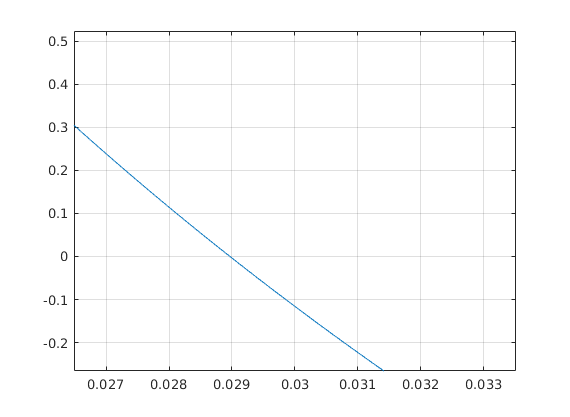
\includegraphics[scale=0.6]{untitled.jpg} \\
	For detailed results, consult the csv file in the project directory.
	
	\section{Discussion}
	From the calculations taken, the pH in the year 1959 was 5.63, and the pH calculated in 2016 was 5.58. While the decline seems small, we must keep in mind that pH is calculated by taking ${log_{10}}{[H^+]}$. This means that the concentration of Hydrogen ions in rainwater has increased over the year, and the trend does not seem to be stopping. In fact this trend can be modeled using the polyfit function in Matlab to give:
	\[pH = -5.523 \times 10^{-6}t^2 + 0.02101t - 14.33\] 
	where t denotes the year. If the trend continues, the pH of rainwater will drop below the threshold of 5.0, creating acid rain.
	\section{Bibliography}
	Data for annual atmospheric levels of \ce{CO2} are taken from: \\
	https://www.esrl.noaa.gov/gmd/ccgg/trends/data.html
	\newpage
	\section{Appendix for Chapter 1}
	\subsection{Code for the bisection method}
	\lstinputlisting{bisectM.m}
	\subsection{Code for processing data}
	\lstinputlisting{Project1.m}

	\chapter{Fluid flows in pipes and tubes}
	\section{Abstract}
	This chapter aims at examining the flow of fluid through pipes and tubes. The project computes the dimensionless \textit{friction factor} in turbulent flows. By computing this factor using the bisection method, the false position method, Newton's method and lastly the fixed point iteration method, this paper draws out comparisons between how effective these methods are and what are the constraints associated with them.
	
	\section{Introduction}
	
	\subsection{Background information}
	Determining the friction factor is of great relevance to many field of engineering and science. Some of these include the flow of liquid and gases through pipelines and cooling systems. Scientists are interested in topics ranging from the flow in blood vessels to nutrient transmission through a plant's vascular system.
	
	\subsection{Problem description}
	In turbulent flows, the \textit{Colebrook equation} provides a means to calculate the friction factor using the equation\\
    \[ 0 =  \frac{1}{\sqrt{f}} + 2.0 \log_{10} \left(\frac{\varepsilon}{3.7D} + \frac{2.51}{\textit{Re}\sqrt{f}}\right) \] \\
    where $\varepsilon$ is the roughness (${m}$), D is the diameter (${m}$), and \textit{Re} is the Reynold's number, as calculated by
    \[\textit{Re} = \frac{\rho V D}{\mu}\]
    where $\rho$ is the fluid's density (${kg/m^{3}}$), V is the velocity (${m/s}$), and ${\mu}$ is the dynamic viscosity (${N.s/m^2}$)
    
	\subsection{Outline}
	By computing Reynold's number using the given values, we can substitute it back into the equation and using the numerical methods discussed, we can find the value of the friction factor. The given values are ${\rho = 1.23 kg/m^3}$, ${\mu = 1.79 \times 10^{-5} N.s/m^2}$, ${D = 0.005 m}$, ${V = 40 m/s}$, and ${\varepsilon = 0.0015 mm}$
	
	\section{Numerical methods}
	The numerical methods involved in the calculation of the friction factor are the bisection method, false position method, Newton's method, and fixed-point iteration method. Consult the attached Matlab project file to see the details of the calculations
	
	\section{Results}
	\subsection{Reynold's number}
    Using Matlab, we are able to determine Reynold's number = ${1.374 \times 10^4}$
    
    \subsection{Plotting graph and estimation}
    Using Matlab to plot the graph, the friction factor seems to be somewhere around 0.029 \\
    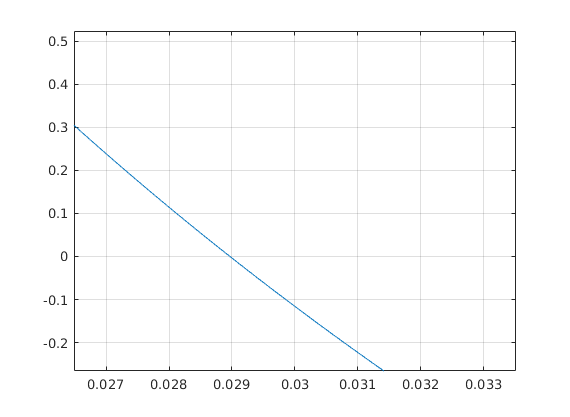
\includegraphics[scale=0.6]{untitled.png}
    
    \subsection{Bisection method and False position method}
    For both of these methods, we approximate the value of the friction factor by using a = 0.008 and b = 0.08, with a tolerance of ${10^{-8}}$
    \subsubsection{Bisection method}
    The bisection method was discussed in chapter 1. For a quick reference as to how this method finds the root of a function, refer to this section in chapter 1 as well as the attached appendix for detailed code in Matlab.\\
    \\
    The method took 26 iterations to calculate the answer. The esitmations converge to 0.02896781 
    \subsubsection{False position method}
    The method of false position combines both the bisection method and the secant method. Starting with the same two initial guesses, the method draws the secant line to find a new estimation for the root, and depending on the sign of the function at the root, the boundaries for root estimation change accordingly. Sample code for the False position method is provided in the appendix. \\
    \\
    The method took 31 iterations to calculate the answer. The estimations converge to 0.02896782
    \subsubsection{Discussion}
    We see that both method converges to the solution, however the bisection method is faster in this case.
    \subsection{Newton's method}
	Newton's method relies on using the tangent line at any point on the function. By finding the intersection of the line with the x-axis, we have a new estimation for the root, with which we can find a new tangent line and repeat the prosess until we find a reasonable estimate for the actual root.    \\
	\\
    We can calculate the derivative of the function quite easily: \\
    \[ h'(f) = \frac{-1}{2 f \sqrt{f}} + 2.0 \left(\frac{log_{10} e \times \frac{-2.51}{2 \textit{Re} f \sqrt{f}}}{\frac{\varepsilon}{3.7D} + \frac{2.51}{\textit{Re}\sqrt{f}}}\right) \]\\
    This is then used for the calculation for Newton's method in the Matlab file provided in the appendix.
    \subsubsection{With initial guess 0.008}
    Took 6 iteration to calculate the answer. The estimations converge to 0.02896781 
    \subsubsection{With initial guess 0.08}
    The approximations do not converge. They fluctuate and eventually go to infinity
    \subsubsection{Discussion}
    We see that Newton's method converges extremely fast if we choose the correct initial guess. This is due to the nature of the function around the root.
    \subsection{Using fzero}
    We use the built-in fzero function with options = optimset('Display','iter', 'TolX', 1e-8).This function searches for a point near the guess where the sign of the function changes
    \subsubsection{With initial guess 0.008}
    The method does not converge to the solution. Complex function value encountered during search
    \subsubsection{With initial guess 0.08}
    The method manages to find an interval [0.0288, 0.116204] where the function changes sign. It then continues to search for the root by evaluating possible values in this interval, and eventually got to f = 0.0289678 
    \subsubsection{Discussion}
    As opposed to Newton's method, fzero was able to find the root with initial guess 0.08, but was unable to do so with initial guess 0.008.
    \subsection{Fixed Point Iteration}
    \subsubsection{Iteration function}
    The fixed point method relies on whether we can find an iteration function ${g(x)}$ such that ${f(x) = x - g(x)}$ and ${|g(xR)| < 1}$ where ${xR}$ is the root of the function. By repeatedly finding ${x}$ for which ${x = g(x)}$, a reasonable estimate for the root is found. The code illustrating this method is attached in the appendix.\\
    \\
    One of the possible iteration functions is: \\
    \[ g(f) = \left(\frac{1}{2.0 \log_{10} \left(\frac{\varepsilon}{3.7D} + \frac{2.51}{\textit{Re}\sqrt{f}}\right)}\right)^2 \]
    \subsubsection{Cobweb Diagrams}
    For initial guess f = 0.008: \\
    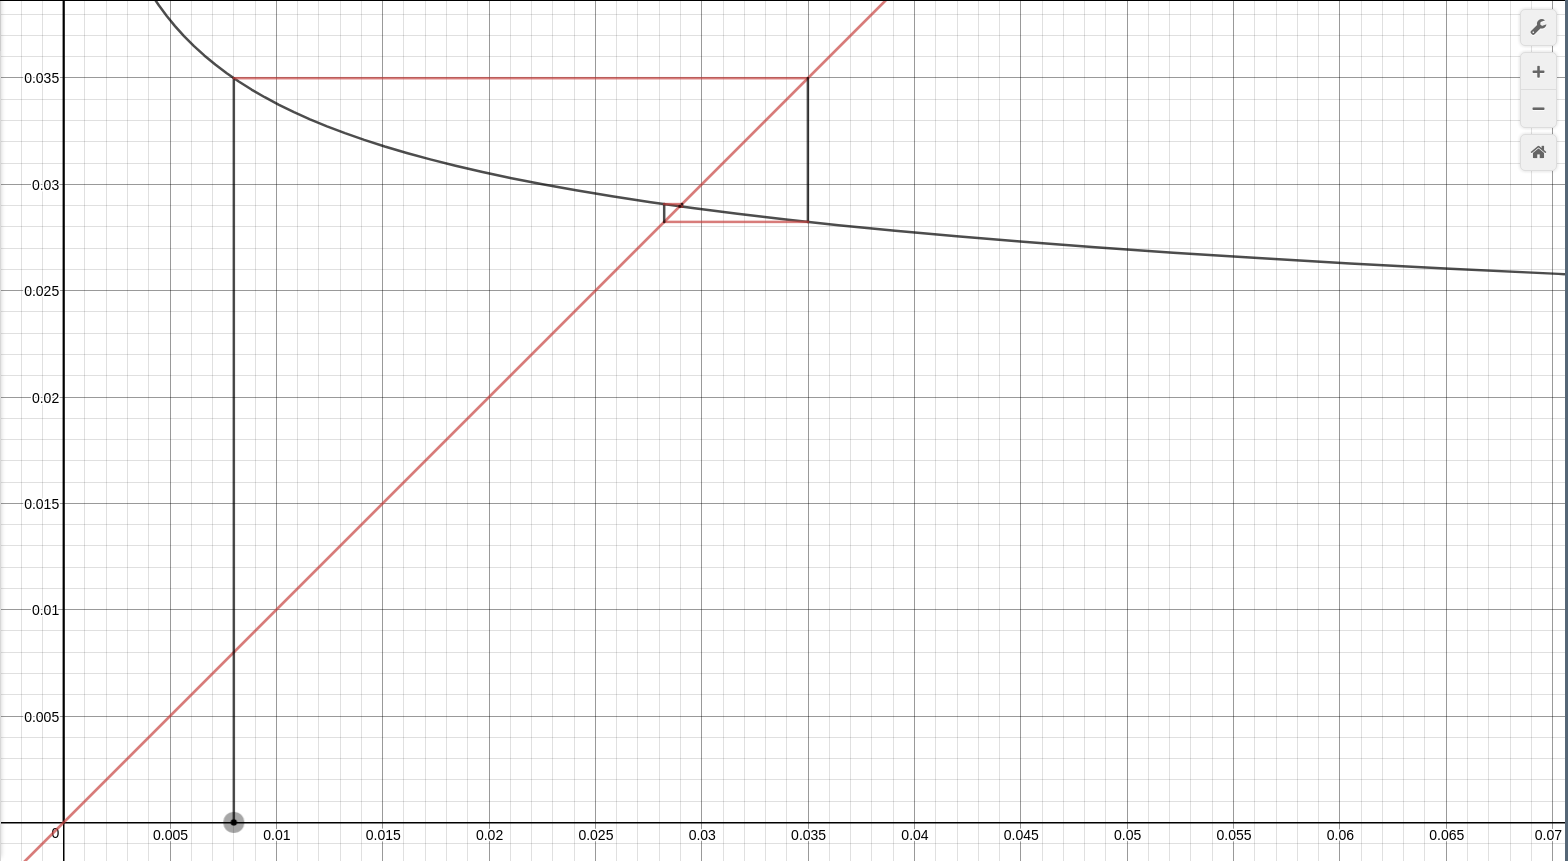
\includegraphics[scale=0.2]{second.png}\\
    For initial guess f = 0.08: \\
    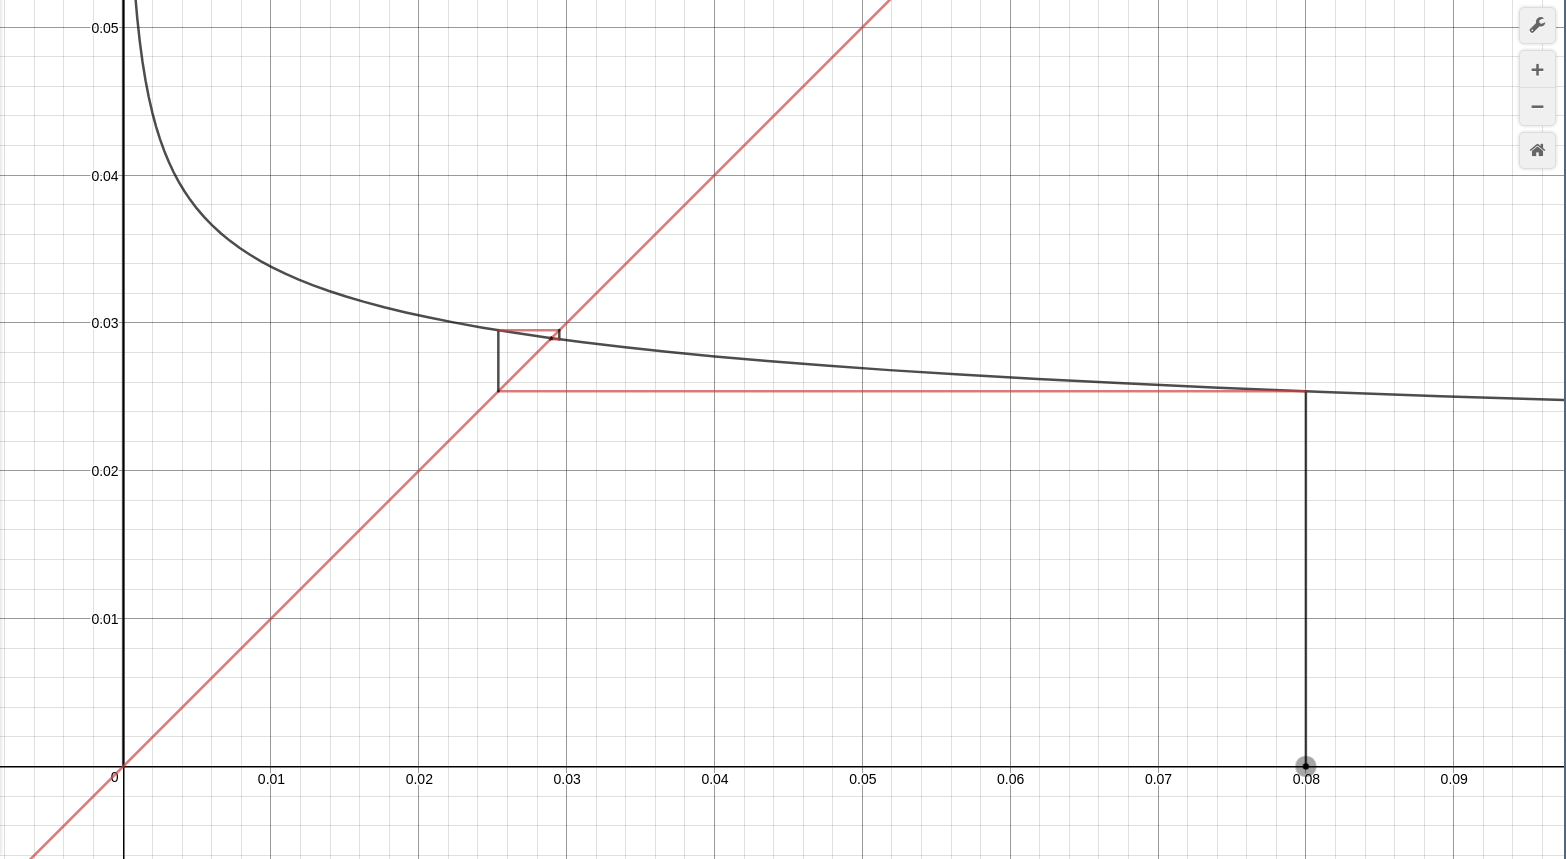
\includegraphics[scale=0.2]{first.png}\\
    \subsection{Discussion}
    With both initial guesses at 0.008 and 0.08, the method was able to find the approximation in 9 iterations. This is because ${|g'(x)| < 1}$ at the root and therefore guarantees convergence.
    \subsection{Appendix for chapter 2}
    \subsection{Code for the false position method}
	\lstinputlisting{falsePositionM.m}
    \subsection{Code for Newton's method}
	\lstinputlisting{NewtonsM.m}
    \subsection{Code for fixed point method}
	\lstinputlisting{fixedpointM.m}
    \subsection{Code for this chapter}
	\lstinputlisting{Project2.m}
	
\end{document}